\section{Introduction}
\label{sec:intro}

Modern software systems expose hundreds to thousands of configuration
options, and the chosen configuration can change performance---execution
time, energy consumption, binary size---by orders of magnitude
\citep{xu2015hey,apel2013feature,pereira2021learning}. For many
engineering tasks the question is not what performance a \emph{typical}
configuration exhibits, but how bad (or how good) performance can get:
worst-case execution time for safety arguments, best-case throughput for
capacity planning, largest kernel size for resource-constrained
deployment. Exhaustive measurement is infeasible even for moderately
sized spaces, so practitioners sample: they measure a budgeted subset of
configurations and use the observed extremum as a proxy for the true
bound.

How trustworthy is such a sampled bound? A recent FSE~2026 study by
\citet{weis2026risk} gives this question a rigorous footing. Building on
scenario theory \citep{calafiore2006scenario,campi2008exact}, it defines
the \emph{posterior risk} of a sampled bound---the empirical probability
that an unseen configuration violates it---and the \emph{posterior
confidence} that the risk stays below a tolerance. These measures are
computed directly from measurements, with no learned model anywhere in
the loop, and they turn strategy comparison into a quantitative exercise:
at the same sample size, which strategy delivers lower risk and higher
confidence? Across five strategies and seven real-world configurable
systems, \citet{weis2026risk} find that Statistical Recursive Search
(\srs) \citep{oh2017srs} ``yields consistently tighter best-case
guarantees---higher posterior confidence and lower posterior risk---than
the alternatives at the same budget,'' while plain solver-based sampling
proves least reliable.

This paper starts from a construct-validity observation about the phrase
\emph{at the same budget}. Like virtually all sampling studies of
configurable systems
\citep{kaltenecker2019distance,pereira2020sampling,guo2018dataefficient},
the FSE study equates budget with \emph{sample size}: strategies are
compared after acquiring the same number of configurations. But
configurations are not interchangeable units of effort. Measuring a
slow, energy-hungry, or large configuration costs more---in wall-clock
time, in joules, in compute dollars---than measuring a cheap one, and
sampling strategies differ systematically in which configurations they
select; indeed, an entire line of strategy design exploits exactly this
asymmetry \citep{sarkar2015cost,nair2017bad}. Whether strategy
\emph{evaluations}, and the recommendations built on them, survive the
switch from counted samples to measured spend has not been examined for
guarantee-oriented sampling---and guarantees are arguably where the
question matters most, because a practitioner who buys a worst-case bound
is typically operating under an explicit measurement budget.

Posterior guarantees are also the sharpest possible place to test such a
cost argument. Studies whose outcome is prediction error entangle the
sampling strategy with a learner, and conclusions can shift with the
choice of regressor \citep{kaltenecker2020interplay}. Posterior risk has
no learner: sample, take the extremum, count violations. Any decision
change we observe when re-indexing by cost is attributable to the cost
construct alone (Figure~\ref{fig:bridge} illustrates the argument).

\begin{figure}[t]
  \centering
  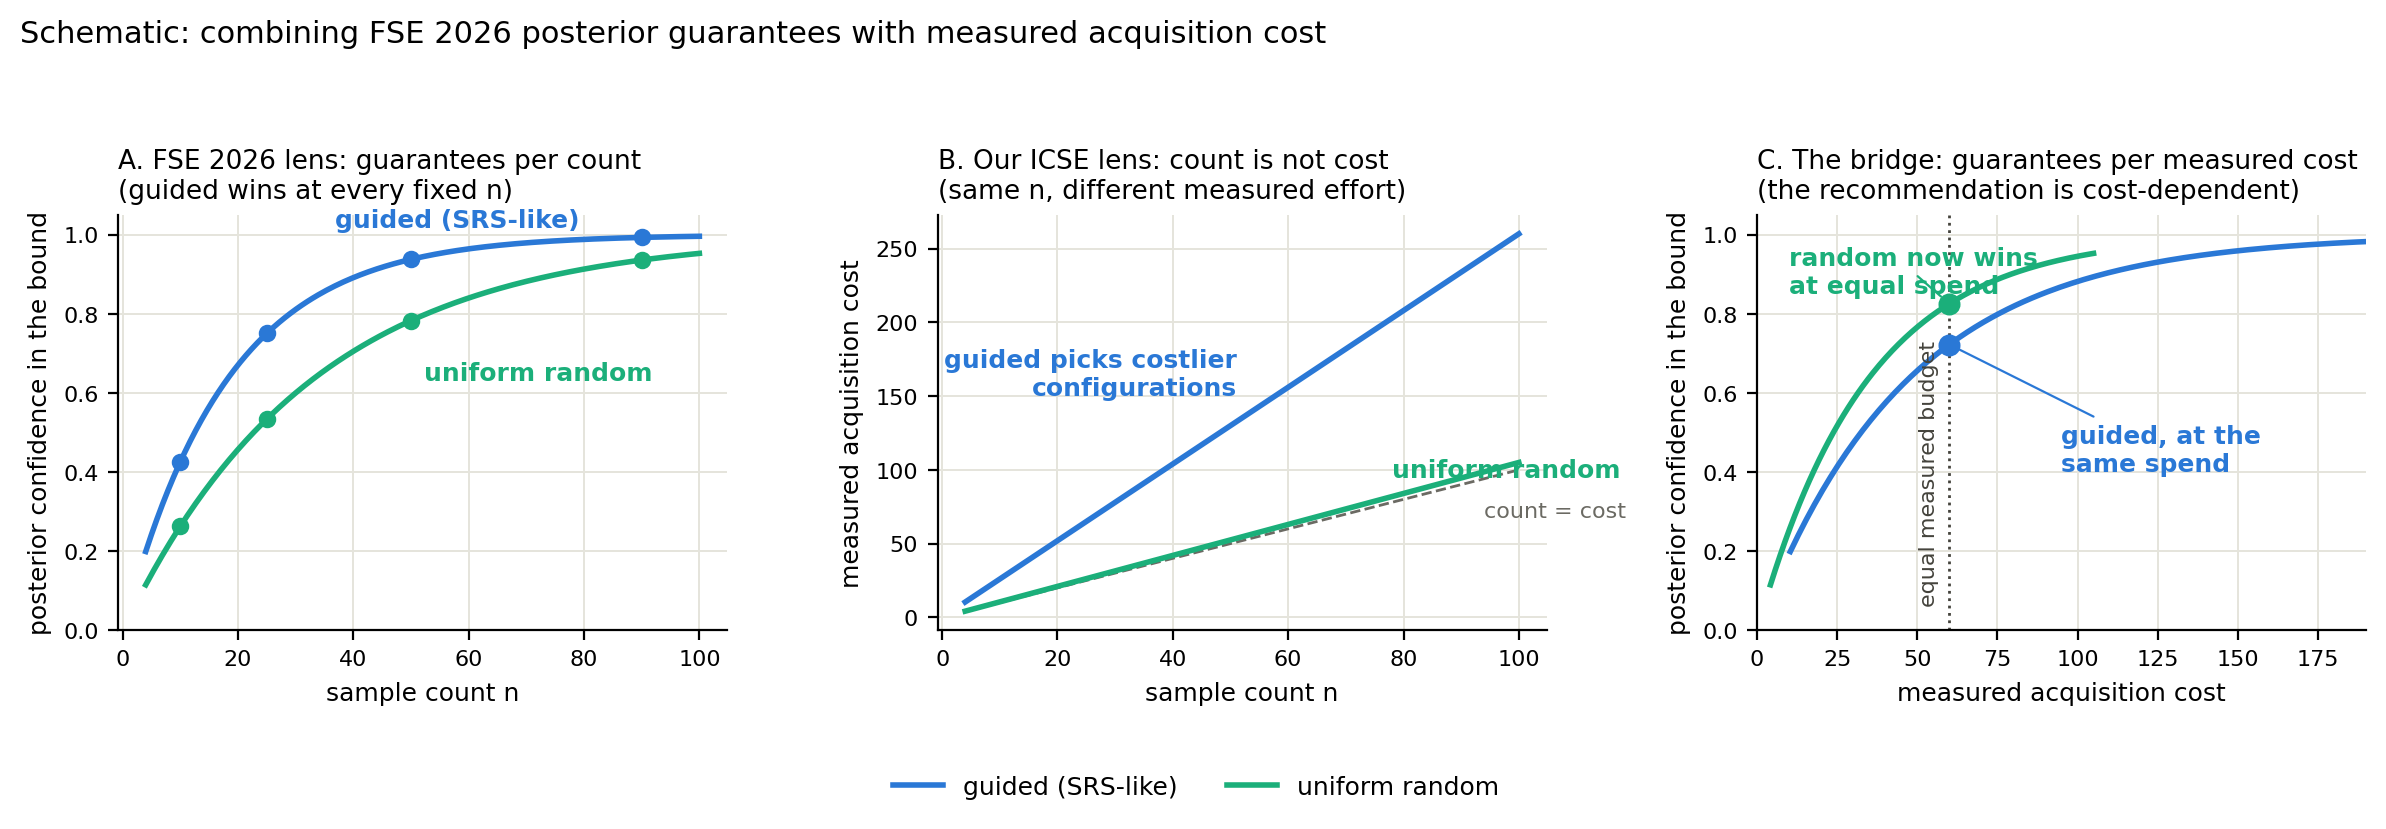
\includegraphics[width=\linewidth]{figures/fig_bridge_concept.png}
  \caption{Schematic of the studied question. (A)~At a fixed sample
  count, a guided strategy such as \srs{} achieves better guarantees than
  uniform random sampling---the FSE~2026 lens. (B)~The same sample count
  can correspond to very different measured acquisition costs.
  (C)~Re-indexing guarantees by measured cost changes the decision
  surface: at an equal measured budget, the recommendation can flip.}
  \label{fig:bridge}
\end{figure}

We therefore conduct a large-scale conceptual replication and extension
of \citet{weis2026risk}, organized around two research questions:

\begin{description}
\item[\rqone:] \emph{Do the FSE~2026 core claims replicate beyond the
  original artifact, at the paper's own fixed-sample-size lens?} We
  decompose this into four sub-questions mirroring the original claims:
  discriminative power of posterior risk, monotone improvement with
  budget, \srs{} superiority, and solver-based unreliability.
\item[\rqtwo:] \emph{Do the FSE~2026 metrics survive re-indexing by
  measured sampling cost instead of sample size?} We decompose this along
  a cost-validity lens: cost heterogeneity at fixed size, calibration of
  size as a cost proxy, impact on recommendations and Pareto frontiers,
  cost-normalized strategy choice, and an explicit equal-spend protocol
  in which strategies literally spend the same measured budget.
\end{description}

Our study spans six corpora: the original FSE artifact (direct data
reuse, seven systems), the x264 corpus of the ICPE'20 replication study
\citep{pereira2020sampling}, fourteen systems with measured energy and
runtime \citep{weber2023twins}, nine systems across all ninety-three
workloads of the ICSE'23 workload study \citep{muehlbauer2023workload},
seven Linux kernel releases \citep{martin2022transfer}, and thirty-five
hyperparameter-optimization pools \citep{zimmer2021autopytorch}---851
(context~$\times$~budget) decision scopes in total.

\paragraph{Findings.} The guarantee \emph{framework} replicates
everywhere: posterior-risk distributions discriminate strategies in
$\approx$95\% of scopes, robust to false-discovery-rate correction. The
strategy \emph{recommendation} replicates only within the original
population: \srs{} dominates on the original systems and on x264, but is
never the best cost-normalized choice on the Linux and
hyperparameter-optimization pools, and rarely so on the energy and
workload families. Under measured cost, the guarantee/cost Pareto
frontier differs from the sample-size frontier in 97.5\% of the 851
scopes---the single most robust effect in our data---while the single top
recommendation changes in 27\%. Two dedicated equal-spend experiments
explain the boundaries mechanistically: a cost-aware strategy designed to
stretch measurement budgets is counterproductive for bounds exactly when
acquisition cost correlates with the target (its equal-spend verdict
flips from $6.6\times$ worse than random to \emph{better} than random as
the coupling weakens), and \srs's advantage requires budget to amortize
(from 4\% of scopes at the smallest budgets to 77\% at the largest).

\paragraph{Contributions.}
\begin{itemize}
\item A conceptual replication of \citet{weis2026risk} at unprecedented
  scale: six corpora, 851 decision scopes, with exact artifact reuse for
  the original systems and an audited reimplementation of \srs{}
  (behaviorally indistinguishable from the artifact, Mann--Whitney
  $p=0.95$).
\item A systematic re-indexing of posterior guarantees by measured
  acquisition cost---a construct-validity question that, to our
  knowledge, had not been examined for guarantee outcomes---at zero
  additional measurement cost, since every corpus already ships the
  required cost data.
\item Two equal-spend experiments (250 scopes) that identify the
  governing mechanisms: cost--target coupling and budget amortization.
  Together they show that ``cost-effective'' is a property of the triple
  (strategy, outcome, cost--target coupling), not of a strategy alone.
\item A fully scripted, checksummed replication package: per-corpus
  result tables, hypothesis tests with false-discovery-rate control, and
  a command-level manifest.
\end{itemize}

The remainder of the paper follows the structure of our research
questions: background and replicated claims
(Section~\ref{sec:background}), study design (Section~\ref{sec:design}),
replication results (Section~\ref{sec:rq1}), cost re-indexing results
(Section~\ref{sec:rq2}), discussion (Section~\ref{sec:discussion}),
threats (Section~\ref{sec:threats}), related work
(Section~\ref{sec:related}), and conclusions
(Section~\ref{sec:conclusion}).
